\documentclass[border=12pt]{standalone}
\usepackage{amsmath, amssymb}
\usepackage{tikz}
\definecolor{ring0}{HTML}{0033CC}
\definecolor{ring1}{HTML}{0066FF}
\definecolor{ring2}{HTML}{0099FF}
\definecolor{ring3}{HTML}{00CCCC}
\definecolor{ring4}{HTML}{00CC66}
\definecolor{ring5}{HTML}{33CC00}
\definecolor{ring6}{HTML}{99CC00}
\definecolor{ring7}{HTML}{CCCC00}
\definecolor{ring8}{HTML}{FF9900}
\definecolor{ring9}{HTML}{FF6600}
\definecolor{ring10}{HTML}{FF3300}
\definecolor{ring11}{HTML}{CC0000}
\definecolor{gap0}{HTML}{E53935}
\definecolor{gap1}{HTML}{1E88E5}
\definecolor{gapfar}{HTML}{CCCCCC}
\begin{document}
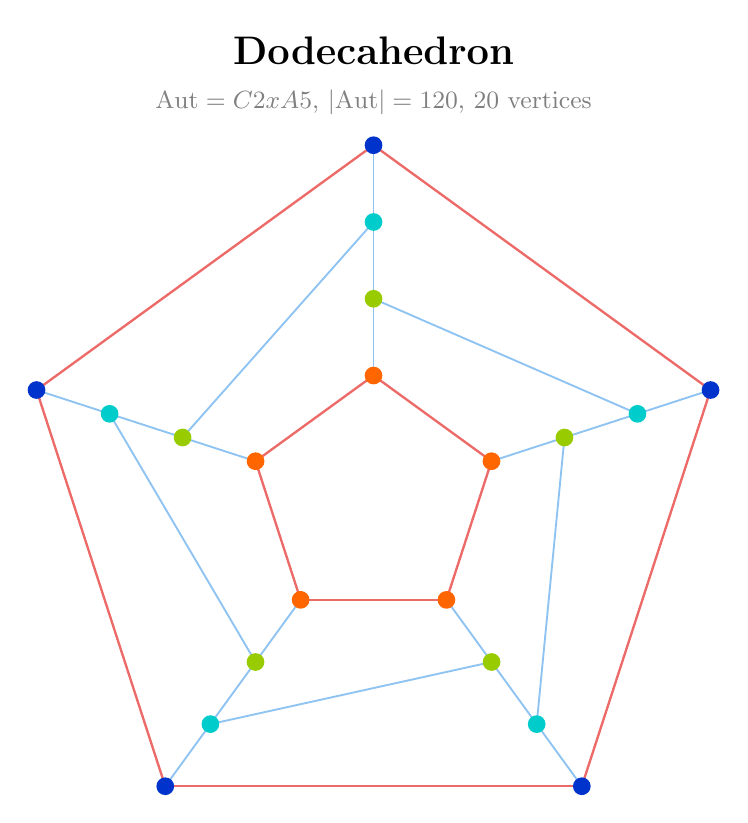
\begin{tikzpicture}
\node[font=\Large\bfseries] at (0, 5.70) {Dodecahedron};
\node[font=\small, text=gray] at (0, 5.05) {$\mathrm{Aut} = C2 x A5$, $|\mathrm{Aut}| = 120$, 20 vertices};
\draw[line width=0.68pt, gap1, opacity=0.50] (0.000, 3.525) -- (0.000, 4.500);
\draw[line width=0.68pt, gap1, opacity=0.50] (0.000, 3.525) -- (0.000, 2.550);
\draw[line width=0.68pt, gap1, opacity=0.50] (0.000, 3.525) -- (-2.425, 0.788);
\draw[line width=0.68pt, gap1, opacity=0.50] (4.280, 1.391) -- (3.352, 1.089);
\draw[line width=0.68pt, gap1, opacity=0.50] (3.352, 1.089) -- (0.000, 2.550);
\draw[line width=0.68pt, gap1, opacity=0.50] (3.352, 1.089) -- (2.425, 0.788);
\draw[line width=0.68pt, gap1, opacity=0.50] (0.000, 2.550) -- (0.000, 1.575);
\draw[line width=0.68pt, gap1, opacity=0.50] (-2.425, 0.788) -- (-3.352, 1.089);
\draw[line width=0.68pt, gap1, opacity=0.50] (-2.425, 0.788) -- (-1.498, 0.487);
\draw[line width=0.68pt, gap1, opacity=0.50] (-3.352, 1.089) -- (-4.280, 1.391);
\draw[line width=0.68pt, gap1, opacity=0.50] (-3.352, 1.089) -- (-1.499, -2.063);
\draw[line width=0.68pt, gap1, opacity=0.50] (-2.645, -3.641) -- (-2.072, -2.852);
\draw[line width=0.68pt, gap1, opacity=0.50] (2.645, -3.641) -- (2.072, -2.852);
\draw[line width=0.68pt, gap1, opacity=0.50] (2.072, -2.852) -- (2.425, 0.788);
\draw[line width=0.68pt, gap1, opacity=0.50] (2.072, -2.852) -- (1.499, -2.063);
\draw[line width=0.68pt, gap1, opacity=0.50] (2.425, 0.788) -- (1.498, 0.487);
\draw[line width=0.68pt, gap1, opacity=0.50] (-1.499, -2.063) -- (-2.072, -2.852);
\draw[line width=0.68pt, gap1, opacity=0.50] (-1.499, -2.063) -- (-0.926, -1.274);
\draw[line width=0.68pt, gap1, opacity=0.50] (-2.072, -2.852) -- (1.499, -2.063);
\draw[line width=0.68pt, gap1, opacity=0.50] (1.499, -2.063) -- (0.926, -1.274);
\draw[line width=0.85pt, gap0, opacity=0.75] (0.000, 4.500) -- (4.280, 1.391);
\draw[line width=0.85pt, gap0, opacity=0.75] (0.000, 4.500) -- (-4.280, 1.391);
\draw[line width=0.85pt, gap0, opacity=0.75] (4.280, 1.391) -- (2.645, -3.641);
\draw[line width=0.85pt, gap0, opacity=0.75] (-4.280, 1.391) -- (-2.645, -3.641);
\draw[line width=0.85pt, gap0, opacity=0.75] (-2.645, -3.641) -- (2.645, -3.641);
\draw[line width=0.85pt, gap0, opacity=0.75] (1.498, 0.487) -- (0.000, 1.575);
\draw[line width=0.85pt, gap0, opacity=0.75] (1.498, 0.487) -- (0.926, -1.274);
\draw[line width=0.85pt, gap0, opacity=0.75] (0.000, 1.575) -- (-1.498, 0.487);
\draw[line width=0.85pt, gap0, opacity=0.75] (-1.498, 0.487) -- (-0.926, -1.274);
\draw[line width=0.85pt, gap0, opacity=0.75] (0.926, -1.274) -- (-0.926, -1.274);
\fill[ring3] (0.000, 3.525) circle (3.2pt);
\fill[ring0] (0.000, 4.500) circle (3.2pt);
\fill[ring0] (4.280, 1.391) circle (3.2pt);
\fill[ring3] (3.352, 1.089) circle (3.2pt);
\fill[ring6] (0.000, 2.550) circle (3.2pt);
\fill[ring6] (-2.425, 0.788) circle (3.2pt);
\fill[ring3] (-3.352, 1.089) circle (3.2pt);
\fill[ring0] (-4.280, 1.391) circle (3.2pt);
\fill[ring0] (-2.645, -3.641) circle (3.2pt);
\fill[ring0] (2.645, -3.641) circle (3.2pt);
\fill[ring3] (2.072, -2.852) circle (3.2pt);
\fill[ring6] (2.425, 0.788) circle (3.2pt);
\fill[ring9] (1.498, 0.487) circle (3.2pt);
\fill[ring9] (0.000, 1.575) circle (3.2pt);
\fill[ring9] (-1.498, 0.487) circle (3.2pt);
\fill[ring6] (-1.499, -2.063) circle (3.2pt);
\fill[ring3] (-2.072, -2.852) circle (3.2pt);
\fill[ring6] (1.499, -2.063) circle (3.2pt);
\fill[ring9] (0.926, -1.274) circle (3.2pt);
\fill[ring9] (-0.926, -1.274) circle (3.2pt);
\end{tikzpicture}
\end{document}